\documentclass[conference]{IEEEtran}
\IEEEoverridecommandlockouts
% The preceding line is only needed to identify funding in the first footnote. If that is unneeded, please comment it out.
\usepackage{cite}
\usepackage{amsmath,amssymb,amsfonts}
\usepackage{algorithmic}
\usepackage{graphicx}
\usepackage{caption}
\usepackage{textcomp}
\usepackage{xcolor}
\usepackage[utf8]{inputenc}
\usepackage{tabularx}
\def\BibTeX{{\rm B\kern-.05em{\sc i\kern-.025em b}\kern-.08em
    T\kern-.1667em\lower.7ex\hbox{E}\kern-.125emX}}
\begin{document}

\title{Desenvolvimento e Aplicação de Drones no Ensino: Uma Abordagem STEAM na Robótica Educacional}

%%\author{Gustavo da Silva Nascimento Costa$^{1}$, João Vitor Nascimento$^{2}$, Jeovana Miranda Souza$^{3}$, Rafael Gomes de \\ Oliveira$^{4}$, Sávio Pessôa Afonso$^{5}$, Rian Cesar Oliveira Souza$^{6}$, Leandro Gonçalves dos Santos$^{7}$, \\and Fábio Santos Lima$^{8}$}

\maketitle
\let\thefootnote\relax\footnote{\\979-8-3315-5288-6/25/\$31.00\textcopyright2025 IEEE}

\begin{abstract}
O projeto Educa Drones, desenvolvido pelo Instituto Federal Baiano - Campus Guanambi, aplica a abordagem STEAM (Ciência, Tecnologia, Engenharia, Artes e Matemática) em um ambiente interdisciplinar de aprendizado prático. Focado no uso de drones de asa rotativa, como o modelo IF450 e as versões Colibri, o projeto permite que estudantes e professores explorem conceitos complexos ao construir e operar essas aeronaves, aplicando-os na pedagogia e em competições estudantis. A iniciativa aprimora o aprendizadoe e incentiva a inovação
\end{abstract}

\begin{IEEEkeywords}
Development and Application of Drones in Education: A STEAM Approach in Educational Robotics
\end{IEEEkeywords}

\section{Introdução}

A educação brasileira, principalmente no ensino básico, apresenta problemas em relação à captação da atenção do aluno e ao estilo de aprendizado e desenvolvimento cognitivo. Essas informações se confirmam ao observar as pesquisas de avaliação.

Os resultados do Programa Internacional de Avaliação de Estudantes (PISA), coordenado pela Organização para a Cooperação e Desenvolvimento Econômico (OCDE), demonstram a defasagem do ensino brasileiro, onde mais de 50\% dos adolescentes de 15 anos não possuem nível básico de conhecimento em matemática, ciências e linguagens \cite{b6}. Essa situação vem se agravando desde 2009.

Em análise, Sassaki et al. \cite{a2} chegaram à conclusão de que grande parte dos avaliados não concluiu a prova, o que se relaciona à dificuldade de entender e solucionar os enunciados, indicando que essa defasagem está mais relacionada a habilidades cognitivas.

Diante desse fato, é necessário buscar meios que incentivem o aprendizado e o desenvolvimento cognitivo dos alunos. A aplicação da metodologia STEAM (acrônimo em inglês para Science, Technology, Engineering, Arts and Mathematics), que funciona por meio da resolução de problemas interdisciplinares, se destaca, especialmente através da robótica, cativando o aluno e fazendo-o aprender por meio da diversão e desafios reais.

Existem diversas maneiras de aplicar a robótica educacional. Um desses recursos pedagógicos, pouco explorados, é a utilização de Aeronaves Remotamente Pilotadas (ARP), popularmente denominadas drones, que permitem que o aluno não apenas crie e opere robôs terrestres, mas também resolva problemas que fugem da bidimensionalidade (XY), permitindo que o estudante dê asas à sua imaginação (XYZ) \cite{a3}.

Além disso, é possível explorar conceitos de física e matemática, como a dinâmica do voo, força, empuxo, leis de Newton, distância, altura, ângulos, trigonometria, entre outros \cite{b11}, conteúdos esses que se mostram difíceis de serem assimilados dentro do paradigma de ensino tradicional.

Por meio da construção desses dispositivos, é possível entender e aplicar conceitos básicos e avançados de eletrônica, química, engenharia e programação \cite{b12}, noções fundamentais para a capacitação de profissionais que serão inseridos em um mercado globalizado. Dessa perspectiva, nasceu no Instituto Federal de Educação, Ciência e Tecnologia Baiano - Campus Guanambi, localizado no sertão produtivo, o projeto Educa Drones, uma iniciativa pioneira no cenário estadual. Promovendo, por meio de oficinas, palestras, competições estudantis, empreendedorismo e inovação tecnológica, um ambiente estimulante e colaborativo para que professores e estudantes se capacitem, troquem experiências e compartilhem ideias que resultem no desenvolvimento de drones e sua inserção no ensino e outros setores que requeiram sua utilização.

Por meio dessa iniciativa, foi possível desenvolver os drones Colibri, que desempenham um papel fundamental na didática e na realização de oficinas, além de contribuir para a participação em competições estudantis. Esses drones possibilitam a divulgação de inovações tecnológicas, a conquista de premiações e a promoção da divulgação científica, da popularização da ciência, do compartilhamento de conhecimento técnico, do fortalecimento de redes de contatos (networking) e do intercâmbio cultural.

Este artigo explora a construção e a implementação dos drones Colibri nas atividades do Educa Drones, realizando uma análise qualitativa de sua aplicação no contexto educacional. Para abordar esses aspectos de maneira mais aprofundada, o artigo está organizado da seguinte forma: a Seção 2 apresenta o Referencial Teórico; a Seção 3 detalha os Materiais e Métodos utilizados; a Seção 4 apresenta os Resultados obtidos; e, por fim, a Seção 6 discute as conclusões do projeto.

\section{Referencial Teórico}

\subsection{Robótica Educacional}

A robótica educativa pode ser definida como uma área do conhecimento multidisciplinar que utiliza os conceitos das engenharias e demais ciências no processo de concepção, construção, automação e controle de dispositivos robóticos com propósitos educacionais \cite{b1}.

A utilização desses recursos tecnológicos com finalidades pedagógicas em instituições de ensino, vem despertando interesse crescente na busca por ferramentas que auxiliem no processo de ensino e aprendizagem \cite{b12}. No que se refere aos drones na educação, deve-se partir do princípio que a educação é um campo em constante evolução e inovação. Entretanto, observa-se uma insuficiência e um processo muito tímido sobre estudos científicos que contemplem a aplicação dos drones no ambiente pedagógico \cite{b9}.

Corroborando com esse entendimento, Yepes \cite{b11} afirma que há muito material sobre robótica educativa, entretanto, são raros os que focam o uso de drones na educação.  Na robótica educacional o drone pode ser utilizado como uma ferramenta de apoio ao ensino, explorando conceitos da física e matemática, tais como dinâmica do voo, força, empuxo e Leis de Newton, distância, altura, ângulos, trigonometria, dentre outros \cite{b11}.

\subsection{Legislação Brasileira Sobre Drones}

De acordo com Regulamento Brasileiro da Aviação Civil (RBAC-E n.94) os drones que possuem peso máximo de decolagem entre 250 g e 25 kg, que operam até 400 pés (cerca de 120 metros) acima do nível do solo e em linha de visada visual (VLOS) são classificados como classe 3 \cite{b2}.

Ainda de acordo com a ANAC, os drones dessa classe não precisam ser de um projeto autorizado ou tipo certificado por esse órgão, ou seja, não é necessário obter certificado de aeronavegabilidade, sendo exigido para sua operação o registro do operador e da aeronave no Sistema de Aeronaves não Tripuladas (SISANT), atender as regras constantes no RBAC-E n.94, assim como a conformidade com Agência Nacional de Telecomunicações (ANATEL) e autorização de voo pelo Departamento de Controle do Espaço Aéreo (DECEA).
\cite{b2}.

\subsection{Competições Estudantis}

Por conseguinte, surgem as competições de drones, tanto no âmbito acadêmico quanto no corporativo, que são um ambiente propício para o emprego da robótica educacional. Dentre elas pode-se citar a Fórmula Drone SAE Brasil,  a Drones IFSC, a Competição Brasileira de Robótica e a mais recente delas, a Competição Baiana de Drones que vai estreiar em setembro de 2025.

A Fórmula Drone SAE Brasil é uma competição de caráter educacional tendo por objeto de interesse técnico o desenvolvimento de uma aeronave de asas rotativas rádio controlada, tipo drone, dotada de sistemas orientados para o cumprimento de determinadas tarefas que constituem o desafio técnico da competição, com foco tecnológico em sistemas inteligentes de bordo \cite{b7}. Foram realizadas três edições (2017, 2018 e 2019) da Fórmula Drones SAE Brasil que ocorreram no Campus da UNIFEI, cidade de Itajubá - MG, e teve sua sequência interrompida pela pandemia do COVID-19. Recentemente, a SAE Brasil divulgou em seu site, a retomada da competição para 2025 que agora tem um novo nome, EletroQuad, e será realizada na Universidade do Vale do Paraíba, em São José dos Campos.

A Competição de Drones do IFSC Campus Florianópolis, é realizada anualmente durante a Semana Nacional de Ciência e Tecnologia (SNCT), ocorrendo desde 2021, tem caráter educacional, com aplicação direta do conceito de STEAM (Science, Technology, Engineering, Arts, Mathematics) em uma atividade de desenvolvimento técnico e tecnológico voltada principalmente para alunos do ensino médio e graduação. O objetivo da competição é estimular os participantes a projetar, montar e pilotar um drone multirotor alimentado à bateria, além de realizar uma série de tarefas atualizadas pelo regulamento todos os anos, que desafiam as habilidades de resolução de tarefas dos participantes e as próprias capacidades técnicas dos veículos. O desempenho dos participantes é julgado através de regras pré-estabelecidas no regulamento da competição \cite{b4}.

A Mostra Nacional de Robótica (MNR) é a maior Mostra Científica de trabalhos de robótica do país. É voltada para alunos do ensino fundamental, médio, técnico e alunos de Graduação, pós-graduação ou pesquisadores da área com o objetivo de estimular, expor e divulgar estudos e a pesquisa na área da Robótica. Os projetos mais bem avaliados concorrem a bolsas de Iniciação Científica Júnior CNPQ/MNR, sendo este projeto, um dos 60 premiados em todo Brasil na edição de 2023 \cite{b5}.

A Competição Brasileira de Robótica (CBR) é composta por 16 categorias que reproduzem problemas do cotidiano, onde robôs autônomos (sem qualquer intervenção humana) devem realizar tarefas corretamente. Entre as categorias, destaca-se a RoboCup Flying Robots League, que é uma modalidade de drones autônomos e inteligentes voltados para inspeção e operação em faixas de dutos e instalações \cite{b3}. Modalidade esta que terá a participação da equipe Drones Guanambi, a qual fará a utilização do drone Colibri Mini, que encontra-se em desenvolvimento e será fruto desse projeto, e que terá sua primeira aparição pública neste evento.

\subsection{Manufatura Aditiva}

A manufatura aditiva é uma ferramenta tecnológica que muito pode contribuir para a aplicação da robótica educacional. Seu conceito foi introduzido em meados da década de 1980 com a disseminação de metodologias de processos de prototipagem rápida, e a impressão tridimensional (3D) era um dos processos possíveis \cite{b10}.

A Impressão 3D é basicamente o ato de transformar uma matéria prima de uma condição física em outra, para produção de um objeto, tomando como base um modelo tridimensional que será materializado pela deposição de camadas \cite{b8}. 

É por meio dessa técnica que os drones citados a seguir são desenvolvidos, possibilitando baratear custos e reproduzir peças caso necessitem de reposição.

\section{Materiais e Métodos}

As aeronaves remotamente pilotadas podem ser do tipo asa fixa ou asa rotativa. Neste estudo nos limitamos ao tipo asa rotativa que também são chamados de multirrotores. Para fins de padronização, nos referimos a essas aeronaves usando o termo drone, como popularmente são conhecidas.

Tendo isso em vista, nesta seção serão explorados a construção da estrutura e a definição dos componentes eletrônicos dos drones desenvolvidos neste subprojeto abarcado pelo projeto Educa Drones. Esses modelos de iniciativa open-hardware foram denominados Colibri Standard, Colibri Lite, Colibri Mini, Colibri Micro e Colibri Hexa.


\subsection{Processo de Construção}

O drone genérico modelo F450 foi o ponto de partida para o desenvolvimento das novas aeronaves. Ele possui quatro braços de plástico injetado, fixados por parafusos em duas placas de fibra de vidro para compor o \textit{frame}. Neste modelo, todos os componentes ficam expostos, a fiação é aparente e a aerodinâmica é prejudicada. Entretanto, apesar dos defeitos, trata-se de uma opção de baixo custo, consideravelmente leve e resistente, sendo amplamente utilizada em competições. 

\begin{figure}[!htb]
    \centering
    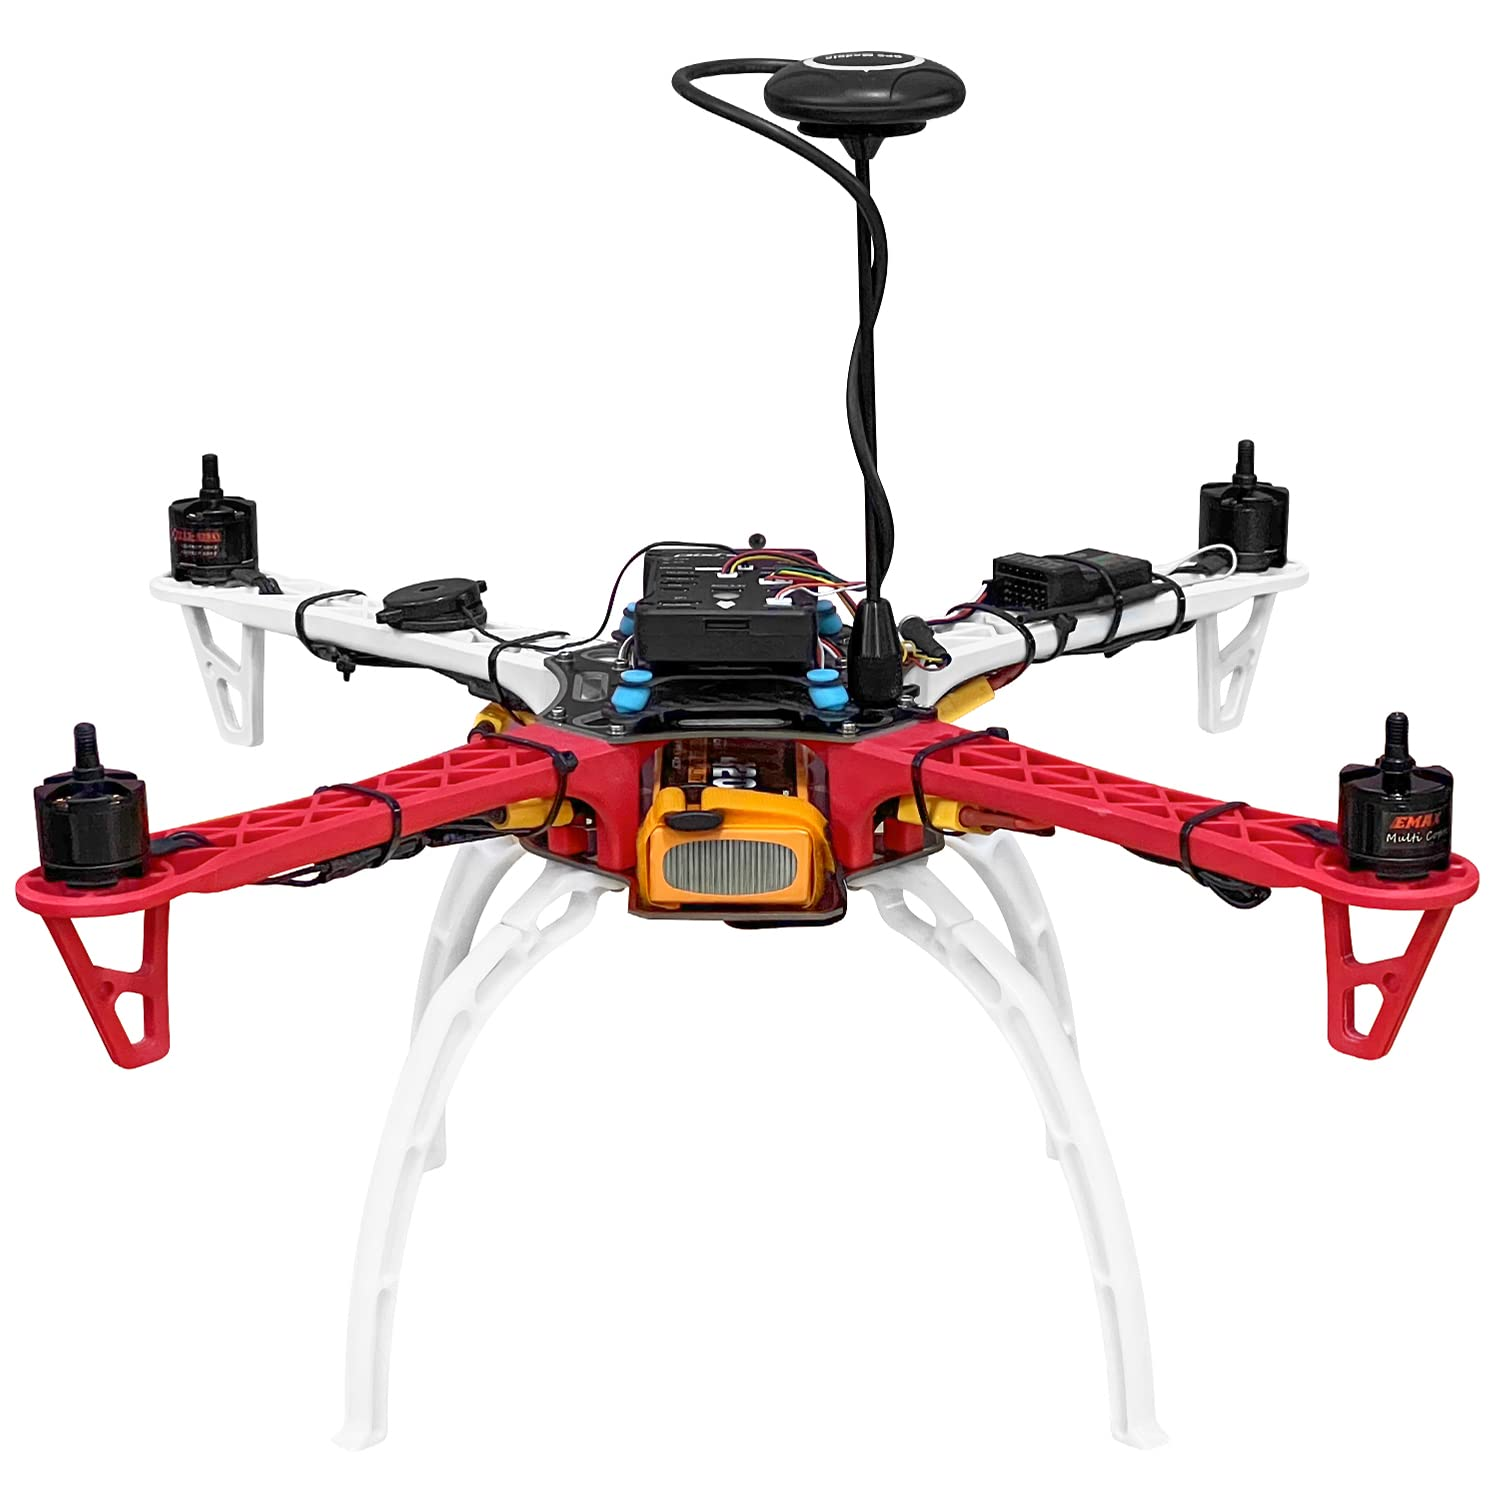
\includegraphics[scale=0.07]{img/f450.jpg} 
    \caption{Imagem do modelo F450 genérico. Fonte: Drones Company.}
    \label{fig:F450}
\end{figure}

Após compreender suas limitações, iniciou-se a modelagem de drones que corrigissem suas falhas e mantendo os pontos positivos. Além disso, foi incluído o critério de modularidade para facilitar a troca de equipamentos, bem como um compartimento seguro e apropriado para o encaixe das baterias. A modelagem tridimensional foi desenvolvida na plataforma Tinkercad, uma ferramenta online gratuita, que pode ser acessado pelo navegador de internet e não exige uma máquina robusta para sua operação.

Após a confecção das peças, O arquivo do projeto foi exportado em formato “.STL" para ser fatiado em camadas, no programa FlashPrint. Ele é responsável por criar o arquivo com extensão “.GX” que é reconhecido pela impressora para realizar a extrusão camada por camada até finalizar a manufatura do objeto projetado.

As novas peças foram impressas em polímero PETG utilizando as impressoras Guider IIs, do fabricante Flash Forge, e a impressora A2v2 Core, da fabricante GTMax3D. O filamento PETG foi escolhido por agregar aos objetos manufaturados, características como durabilidade, tenacidade, flexibilidade, leveza e resistência à impactos.

\subsection{Modelo Colibri Standard}

O drone recebe o nome de um beija-flor: Colibri, em homenagem à cidade de Guanambi (beija-flor em Tupi), tendo seu sufixo standard (“padrão” em inglês) por ser o modelo de referência para as demais versões. O formato do corpo central do frame foi inspirado no F450 genérico, entretanto com algumas modificações estratégicas para melhor acomodar os componentes eletrônicos (figura \ref{fig:F450}).

\begin{figure}[!htb]
    \centering
    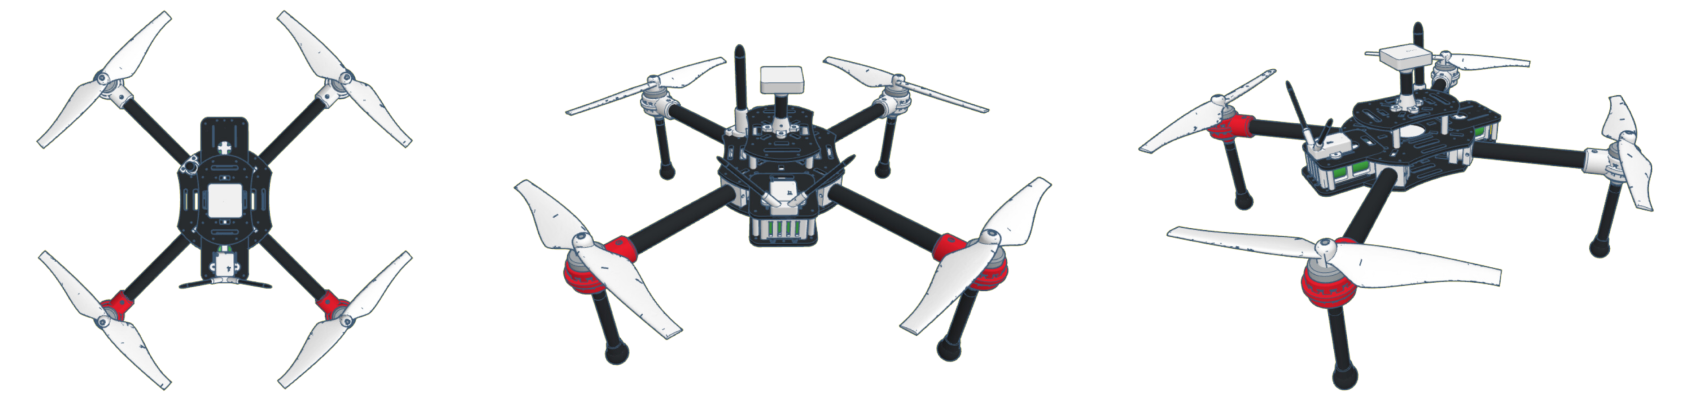
\includegraphics[scale=0.14]{img/Colibri-standard.png} 
    \caption{Modelo tridimensional do drone Colibri Standard no TinkerCad. Fonte: Autor}
    \label{fig:ColibriStandard}
\end{figure}

Ele mantém a distância de 450 mm entre os eixos e um centro de formato similar, utilizando braços tubulares de fibra de carbono de 16 mm, o que proporciona resistência e proteção para fios e dispositivos que podem ser inseridos em seu interior. O trem de pouso também é produzido com tubos de fibra de carbono, com 12 mm de diâmetro e 1 mm de espessura. 

Além disso, possui diversas furações previamente definidas que permitem a integração de variados acessórios como sensores e mecanismos robóticos.

\subsection{Modelo Colibri Lite}

O Colibri Lite possui as mesmas dimensões entre os eixos dos rotores de sua versão \textit{Standard}, porém com modificações na estrutura do corpo central priorizando a redução de peso. Ele foi planejado para competições nas quais o peso influencia significativamente na pontuação, mas que não permitem drones de dimensões menores.

\begin{figure}[!htb]
    \centering
    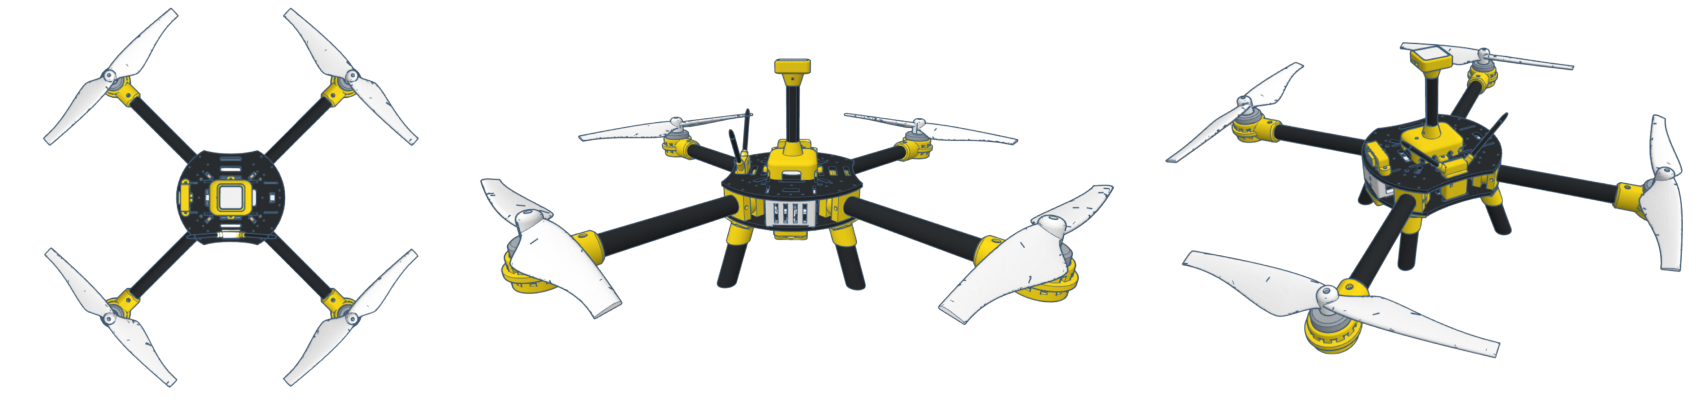
\includegraphics[scale=0.14]{img/Colibri-lite.png} 
    \caption{Modelo tridimensional do drone Colibri Lite no TinkerCad. Fonte: Autor}
    \label{fig:my_label}
\end{figure}

\subsection{Modelo Colibri Mini}
O Colibri Mini é um modelo que possui 330 mm entre os eixos dos motores. Ele apresenta braços de fibra de carbono tubulares de 12 mm de diâmetro e 1 mm de espessura, tratando-se de forma geral, um modelo em escala reduzida do Colibri Lite. 

Seu desenvolvimento foi iniciado pensando na utilização em competições onde apenas é permitido drones de tamanhos inferiores a 450 mm. Mesmo tendo por padrão 330 mm, essa dimensão pode ser modificada de acordo com a necessidade.

\begin{figure}[!htb]
    \centering
    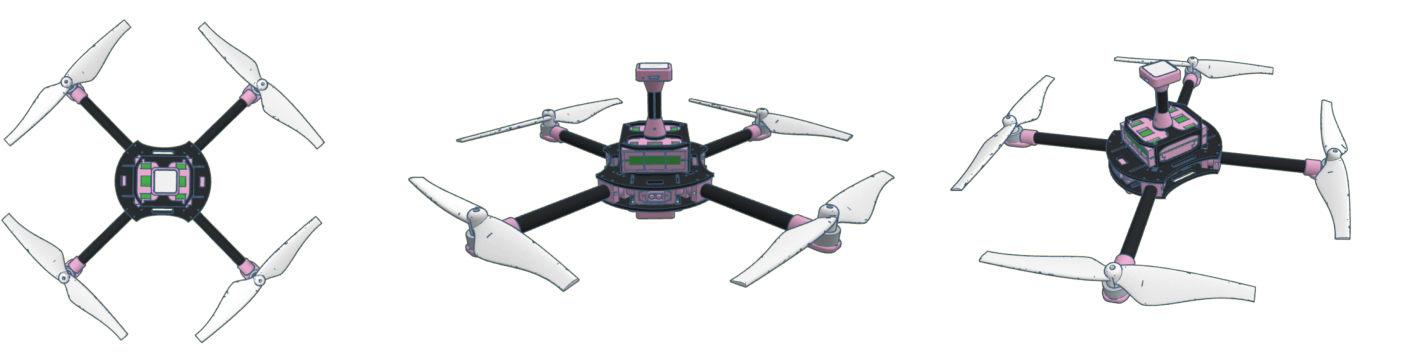
\includegraphics[scale=0.14]{img/Colibri-mini.png} 
    \caption{Modelo tridimensional do drone Colibri Mini no TinkerCad. Fonte: Autor}
    \label{fig:ColibriMini}
\end{figure}

\subsection{Modelo Colibri Micro}

O Colibri Micro é o modelo mais compacto e leve da série Colibri, com uma distância de 188 mm entre os eixos dos motores. Ele é o único a apresentar estrutura inteiramente feita por manufatura aditiva.

Desenvolvido para missões aéreas em locais fechados ou com demasiado obstáculos, onde sua proteção de hélice robusta e integrada nativamente permite menor vulnerabilidade a avarias e maior segurança à animais e pessoas

\begin{figure}[!htb]
    \centering
    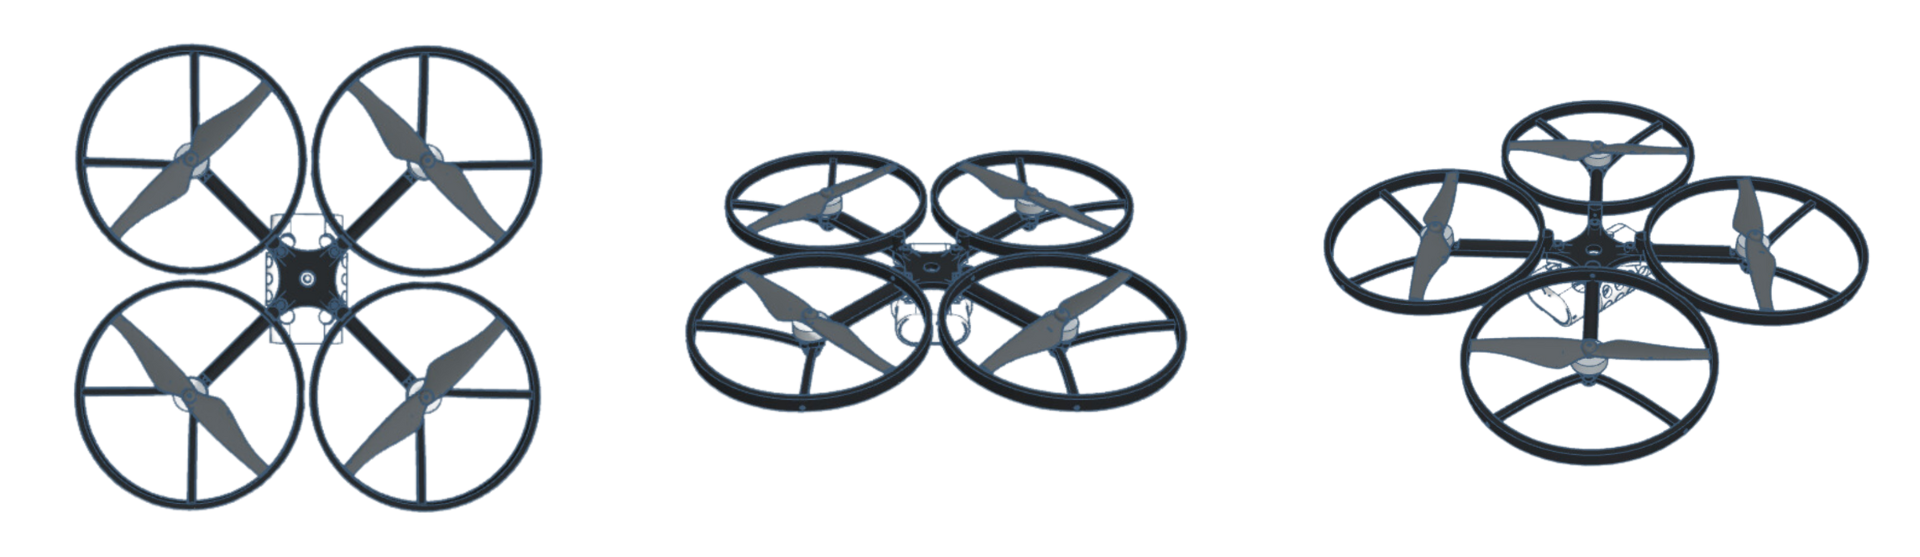
\includegraphics[scale=0.12]{img/Colibri-micro.png} 
    \caption{Modelo tridimensional do drone Colibri Micro no TinkerCad. Fonte: Autor}
    \label{fig:my_label}
\end{figure}

\subsection{Modelo Colibri Hexa}
O Colibri-Hexa é o maior de sua linha, com 6 rotores e 550mm de distância entre os opostos e 60° entre cada braço subsequente. Assim como nas outras versões, esse modelo possui braços tubulares de fibra de carbono com 16 mm de diâmetro.

\begin{figure}[!htb]
    \centering
    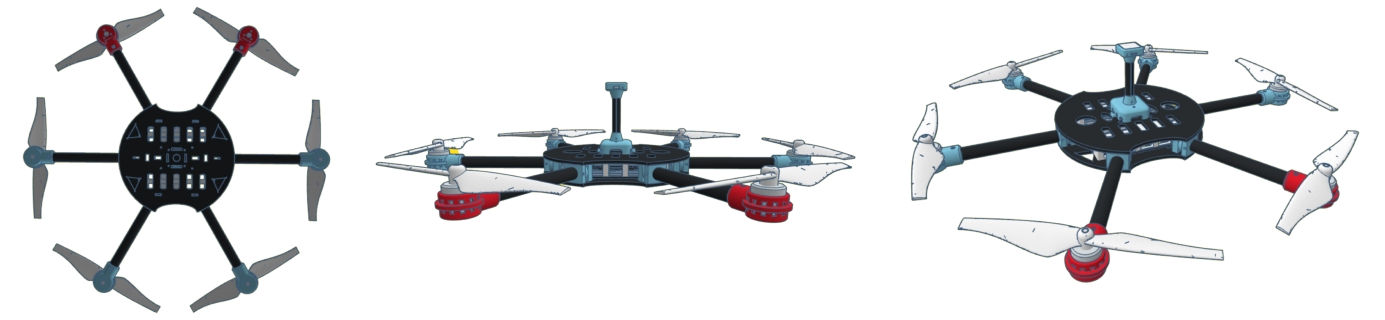
\includegraphics[scale=0.14]{img/Colibri-hexa.png} 
    \caption{Modelo tridimensional do drone Colibri Hexa no TinkerCad. Fonte: Autor}
    \label{fig:my_label}
\end{figure}

A existência de seis motores proporciona ao drone maior estabilidade e redundância, permitindo que a aeronave permaneça em voo mesmo com a falha de um deles. Ademais, ela é capaz de operar com peso adicional, o que possibilita a integração de equipamentos mais robustos.

\subsection{Componentes Eletrônicos}

Esse tópico aborda brevemente e de forma mais técnica o sistema de propulsão, controladoras de voo, sensores integrados e outros componentes essenciais que contribuem para a funcionalidade e desempenho dessas aeronaves não tripuladas.

Todas as versões de drones desenvolvidas compartilham componentes eletrônicos semelhantes, como o Electronic Speed Control (ESC), que utiliza o firmware BLHeli ou SimonK, e é conectado a uma controladora de voo de 32 bits configurada com o firmware Ardupilot.

Quanto aos rotores, são utilizados motores brushless de 800 KV, 1400 KV e 2824 KV, os quais possuem relação inversamente proporcional ao tamanho da estrutura e da hélice.

Todas as baterias são desenvolvidas de maneira personalizada para cada modelo, utilizando células de íon de lítio de capacidade variada e tensão nominal de 3,7 volts.

Para telemetria, todas as versões utilizam o módulo ESP32 executando o firmware Drone Bridge. Em combinação com um roteador WiFi de 2,4 GHz, essa configuração permite uma comunicação MAVLink bidirecional e criptografada entre o drone e a estação de controle (computador ou smartphone).

O sistema de posicionamento GNSS utilizado em todas as versões é embarcado com o chip receptor Ublox-M10050 e sensor magnético QMC5883L. Esse sistema opera com frequência mais alta do que o normal e suporta todos os sinais GNSS L1 (GPS, GLONASS, Galileo, BeiDou), sendo três destes simultaneamente e pode usar até 32 satélites para navegação com taxa de atualização de 10 Hz.

\section{Resultados e Discussões}

\subsection{Desempenho das Aeronaves}

\begin{table}[htbp]
\centering
\caption{Comparação dos Modelos de Drones}
\label{tab:drone_comparison}
\begin{tabularx}{\columnwidth}{|l|X|X|X|}
\hline
\textbf{Modelo}         & \textbf{Peso Operacional} & \textbf{Tempo de voo} & \textbf{Telemetria (raio)} \\ \hline
Colibri Standard       & 1040 g                    & 28 min               & +300 m                     \\ \hline
Colibri Lite           & 788 g                     & 12 min               & +300 m                     \\ \hline
Colibri Mini           & 501 g                     & 28 min               & +300 m                     \\ \hline
Colibri Micro          & 275 g*                    & -                    & +300 m                     \\ \hline
Colibri Hexa           & -                         & -                    & +300 m                     \\ \hline
\end{tabularx}
\newline
\small *Peso estimado
\end{table}

O modelo Stansard apresenta o maior peso dentre os drones de 450mm testados, com 1040 gramas. Em contrapartida, o Lite é o mais leve entre os drones da classe 450, pesando 788 g. A redução de peso é um fator crítico, especialmente em competições onde a leveza pode melhorar significativamente a pontuação. Para competições onde o tamanho da aeronave não é limitante, as versões Colibri Mini, Micro e Hexa se tornam uma ótima alternativa, sendo os dois primeiros pensados em competições em ambientes fechados com múltiplos obstáculos e o último onde o carregamento de carga e estabilidade de voo se torna crucial para uma boa pontuação.

Entre os drones da classe 450, o Colibri Standard  apresentou o maior tempo de voo, com 28 minutos. Em contraste, o Colibri Lite tem um tempo de voo significativamente menor, de apenas 12 minutos, devido à sua bateria de menor capacidade. O Colibri Mini também apresentou 28 minutos voo mesmo tendo uma bateria menor. O motivo é que seu peso é 34,3\% menor que o do Colibri Standard. 

Todos os modelos apresentam uma capacidade de alcance de telemetria de +300 m, indicando uma comunicação robusta o suficiente para a maioria das aplicações de campo. Este alcance é adequado para operações de áreas inferiores a 9 hectares.

\subsection{Aplicação Pedagógica}

A utilização pedagógica dos drones desenvolvidos foi implementada por meio de feiras, mostras, workshops e treinamentos, muitas vezes conduzidos pelos próprios alunos participantes do projeto, como uma forma de aprendizado mútuo.

Por meio de atividades de pesquisa e ensino, os alunos do campus Guanambi, têm a oportunidade de trabalhar em atividades de desenvolvimento tecnológico, como o presente estudo. Essas iniciativas incentivam os estudantes a se aprofundarem nas ciências exatas e naturais de forma espontânea e orgânica.

Um dos resultados desse incentivo ocorreu em 2023, quando foi concedida a um aluno  do ensino médio do instituto, participante do projeto Educa Drones, uma bolsa de iniciação científica da Mostra Nacional de Robótica. Demonstrando a qualidade do ensino quando potencializado por recursos pedagógicos.

\begin{figure}[!htb]
    \centering
    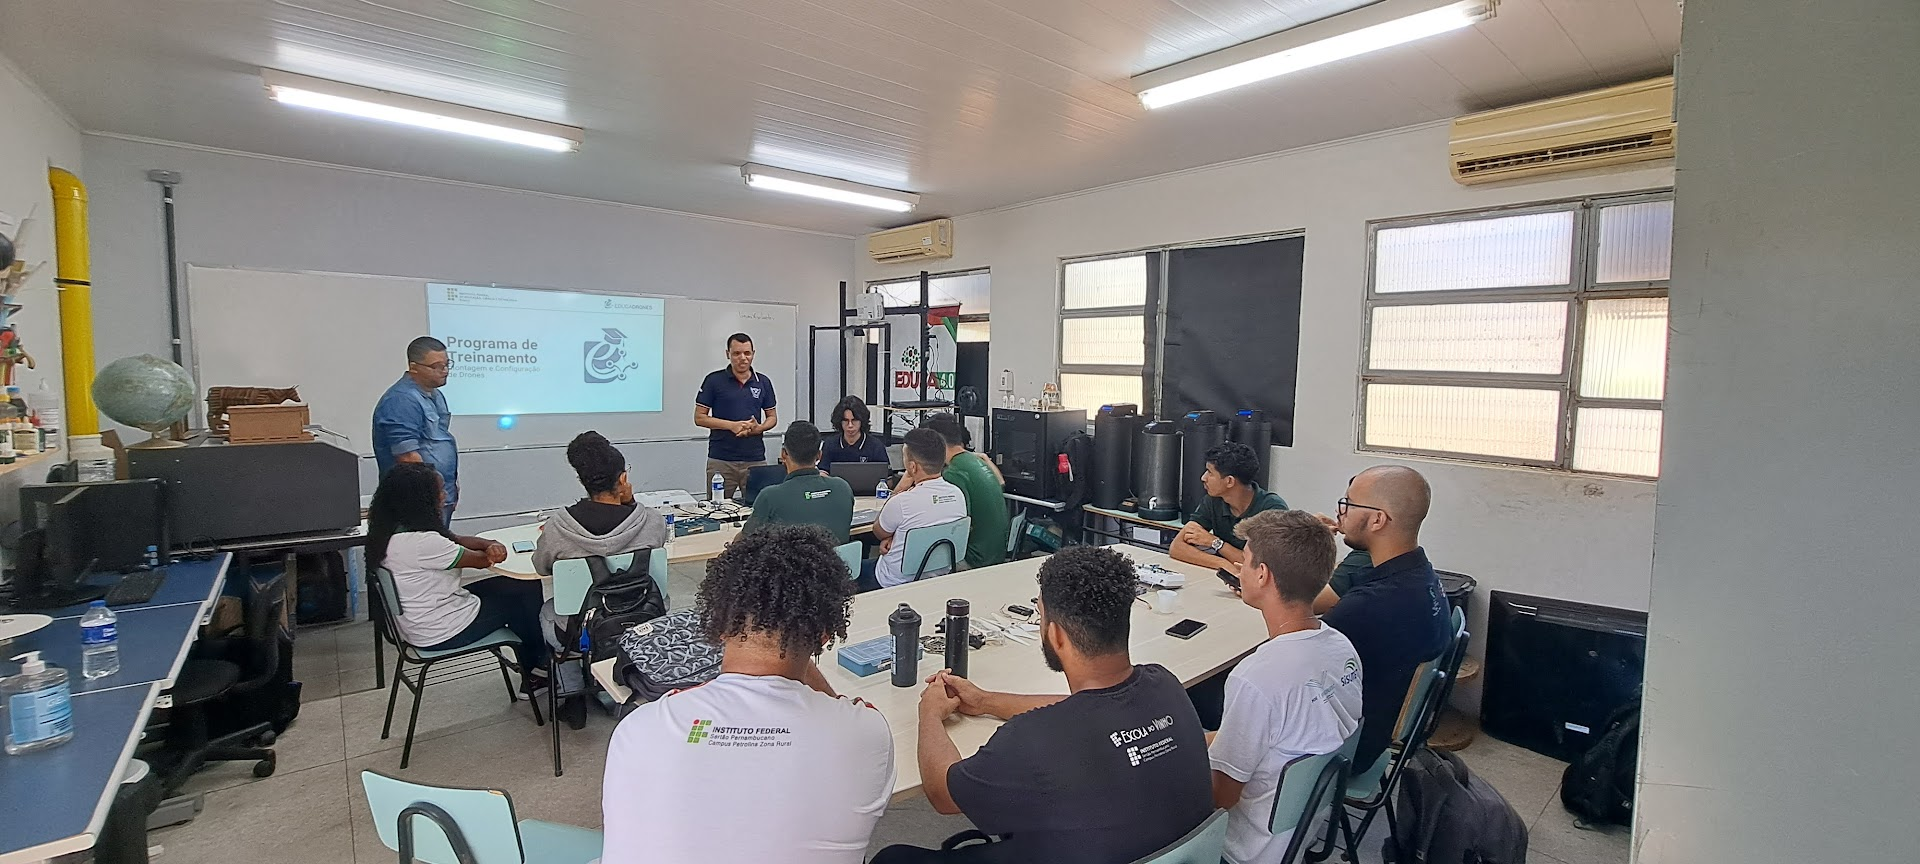
\includegraphics[scale=0.12]{img/petrolina.jpg} 
    \caption{Treinamento de Montagem e Configurações de Drones em Petrolina-PE. Fonte: Autor}
    \label{fig:petrolina}
\end{figure}

 Destaca-se ainda, o programa de treinamento "Montagem e Configurações de Drones", ministrado pelo professor do IF Baiano Campus Guanambi, Leandro G. dos Santos, e por alunos experientes na montagem de aeronaves. O objetivo é fomentar a inovação em sistemas de aeronaves remotamente pilotadas (RPAS) nos diversos campi do IF Baiano, com implementações já realizadas nos campi de Catu-BA, Alagoinhas-BA, e Petrolina Zona Rural (figura \ref{fig:petrolina}), do Instituto Federal do Sertão Pernambucano. O curso também é regularmente oferecido no campus de origem, com planos de expandir para outros unidades da Rede Federal e demais instituições interessadas.

Voltado para alunos do ensino médio e graduação, esse curso do programa de treinamento adota a metodologia STEAM, abordando a legislação, aplicação, montagem e configuração de drones, integrando teoria e prática de forma didática.

Para manter o interesse dos participantes dos eventos promovidos pelo projeto, a participação em competições, como a Olimpíada Nacional de Drones Aeromodelos (ONdDA), é incentivada. A primeira edição dessa competição ocorrerá em 2025. Além de benéfico para os alunos, que têm a possibilidade de conhecer e aprender com outros participantes, incentiva a criação de inovações e o desenvolvimento científico no país. 

Ademais, o IF Baiano campus Guanambi, procura viabilizar uma competição interna, que reunirá todas as instituições que participaram do programa de treinamento e outras que tiverem interesse, com o objetivo de por em prática conhecimentos presentes na metodologia STEAM, como lançamento horizontal, cálculo de área e perímetro, visão computacional, eficiência energética, aerodinâmica, entre outros.

\subsection{Aplicação em Competições Estudantis}

A participação dos estudantes em competições estudantis, além de possibilitar a divulgação de suas inovações e conquista de premiações, também proporcionam a divulgação científica, a popularização da ciência, o compartilhamento de conhecimento técnico, network e intercâmbio cultural. Por conseguinte, essa articulação interdisciplinar favorece positivamente no processo de ensino-aprendizagem contribuindo na formação acadêmica e cidadã dos estudantes.

\begin{figure}[!htb]
    \centering
    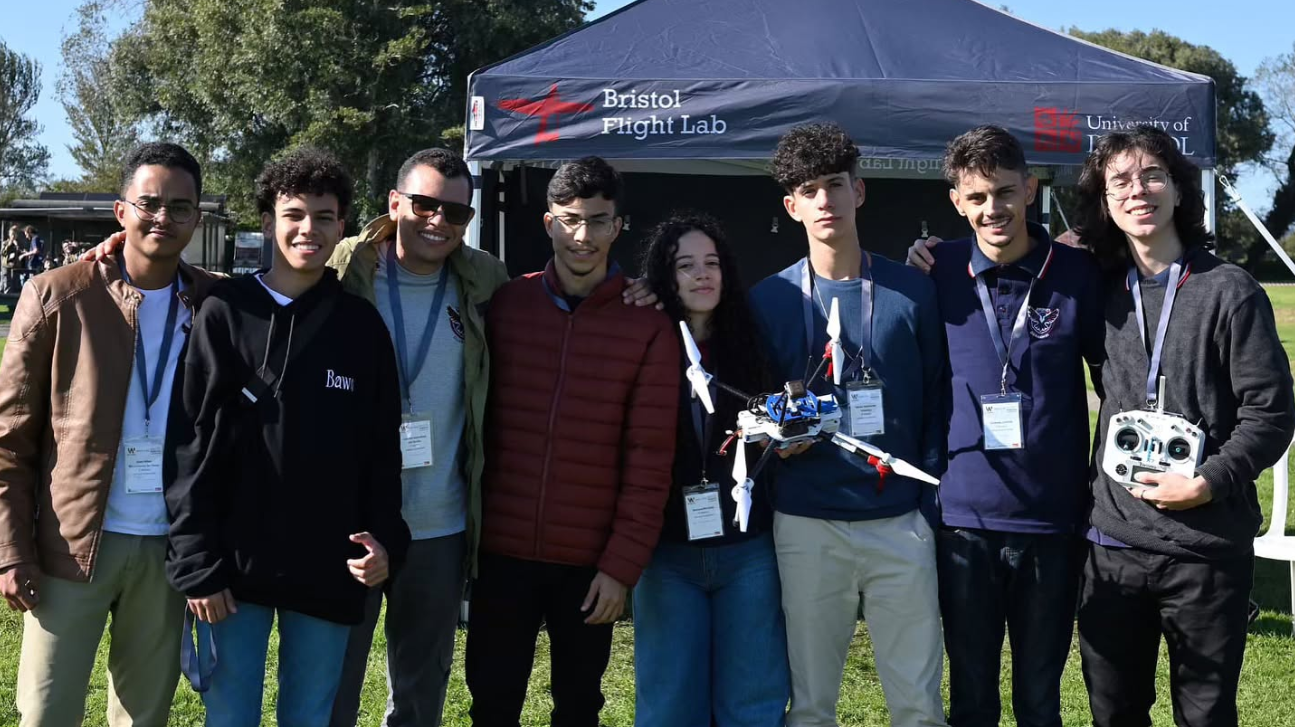
\includegraphics[scale=0.30]{img/imav2024.png} 
    \caption{Equipe Drones Guanambi na competição outdoor da IMAV. Fonte: Autor}
    \label{fig:imav}
\end{figure}

Como exemplo, o desenvolvimento dos diferentes modelos de drones apresentados nesse estudo, integrado a elaboração do artigo "Comparative analysis of cameras for ArUco marker recognition in Unmanned Aerial Vehicles"\cite{a1}, credenciou a participação de estudantes do IF Baiano Campus Guanambi no evento \textit{International Micro Aerial Vehicles Competition} (figura \ref{fig:imav}) de 2024, onde o Colibri Standard (figura \ref{fig:ColibriStandard}) foi utilizado pela equipe Drones Guanambi.

\begin{figure}[!htb]
    \centering
    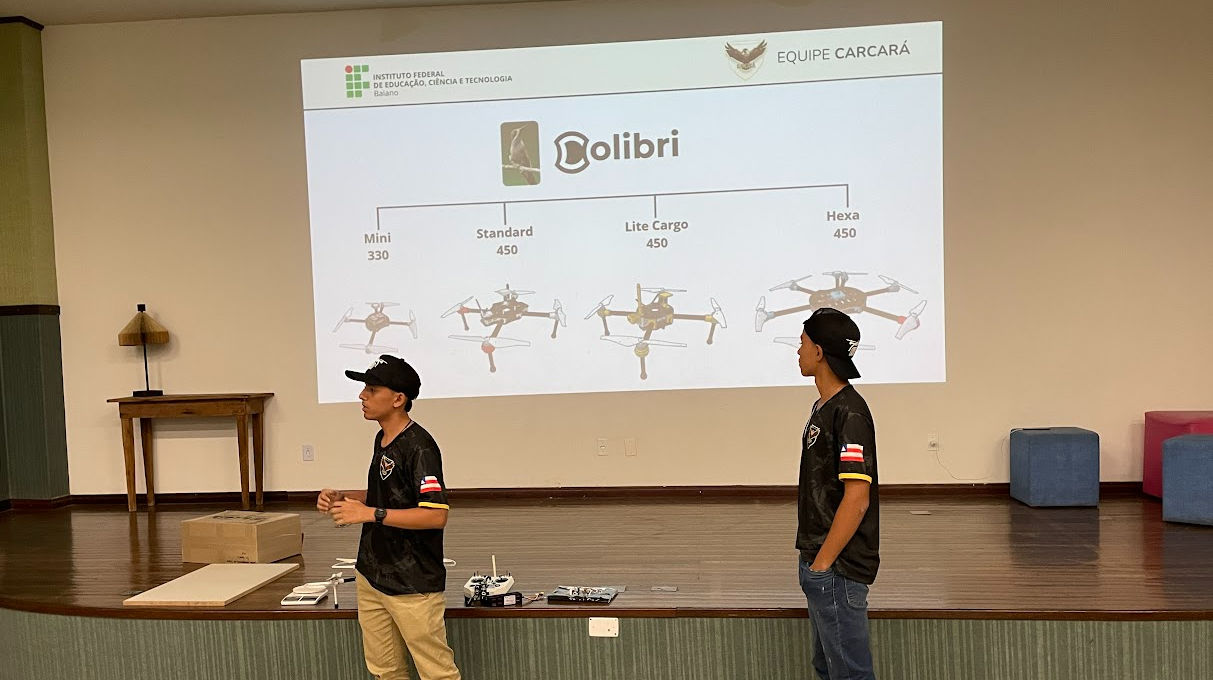
\includegraphics[scale=0.30]{img/ifsc.png} 
    \caption{Apresentação técnica dos drones Colibri durante a competição Drones IFSC. Fonte: Autor}
    \label{fig:ifsc}
\end{figure}

Na competição "Drones IFSC", realizada em Florianópolis no ano de 2024, os estudantes do IF Baiano Campus Guanambi, estreiaram o drone Colibri Cargo, o qual despertou a atenção dos demais competidores e dos jurados (figura \ref{fig:ifsc}), pelo design inovador e elevada capacidade de transporte de carga, finalizando o evento com a conquista do terceiro lugar no pódio.

Em adição, os desafios propostos nessas disputas fomentam o desenvolvimento tecnologico do país, incentivando os discentes a criarem soluções econômicas para problemas reais, que, ao serem aprimoradas, permitem a inserção no meio comercial.

\section*{Considerações Finais}

Destaca-se as características distintivas de cada modelo de drone desenvolvido no projeto Educa Drones, evidenciando suas aplicações ideais com base em peso, tempo de voo e capacidades de telemetria. O desenvolvimento contínuo e a avaliação desses drones podem levar a melhorias significativas na eficiência e versatilidade dos veículos aéreos não tripulados.

Para conclusões mais abrangentes, são necessários dados adicionais dos modelos Colibri Micro e Colibri Hexa. Investigações futuras devem focar na coleta desses dados, bem como nas análises de resistência, peso máximo de decolagem e estabilidade e voo em condições de vento adversas. Além disso, a comparação com outros drones comerciais pode fornecer uma perspectiva mais ampla sobre a competitividade dos modelos desenvolvidos.

As competições nas quais se participou, mostraram as qualidades e defeitos dos modelos utilizados,  permitindo a analise de pontos de fragilidade, incluindo a substituição da atual telemetria por outras mais resistentes a falhas.

Voltado para as aplicações pedagógicas e competições estudantis previstas para 2025, a utilização dos drones aqui descritos, tanto da Olimpíada Nacional de Drones Aeromodelos quanto na competição interna, permitirá maior observação prática dos reais efeitos dos programas de extensão e sua contribuição na formação dos estudantes envolvidos.

\begin{thebibliography}{00}
\bibitem{b1} Abreu, J. V. V.; Bastos, B. L. (2015). Robótica Pedagógica e Currículo do Ensino Fundamental: Atuação em uma Escola Municipal do Projeto UCA. Revista Brasileira de Informática na Educação, v.23, n.3, 2015

\bibitem{b2} Brasil. Agência Nacional de Aviação Civil. (2023). Requisitos gerais para aeronaves não tripuladas de uso civil. RBAC-E94. Emenda n.3. Brasília, 2023.

\bibitem{b3} CBR, Competição Brasileira de Robótica. Disponível em: <https://cbr.robocup.org.br/index.php/categorias/> Acessado em de 30 junho 2024.

\bibitem{b4} IFSC, Competição de Drones IFSC Câmpus Florianópolis. Disponível em: <https://www.ifsc.edu.br/web/campus-florianopolis/veiculos-nao-tripulados-competicao-de-drones> Acessado em de 30 junho 2024.

\bibitem{a1} L. G. dos Santos, J. V. N. Souza, D. F. S. Junio, R. G. de Oliveira, S. P. Afonso, J. M. Souza, F. S. Lima, and R. M. Cotrim, “Comparative analysis of cameras for aruco marker recognition in unmanned aerial vehicles,” in 15$^{th}$ annual international micro air vehicle conference and competition, Bristol, United Kingdom, 2024, p. 177–184.

\bibitem{b5} MNR, Mostra Nacional de Robótica. Disponível em: <https://mnr.robocup.org.br/> Acessado em de 30 junho 2024.

\bibitem{b6} OECD. PISA 2022 Results (Volume I): The State of Learning and Equity in Education. Paris: OCDE Publishing, 2023.

\bibitem{b7} SAE BRASIL. (2020). Fórmula Drone. Disponível em: <http://portal.saebrasil.org.br/programas-estudantis/sae-brasil-helidesign> Acesso: 20 de junho de 2020.

\bibitem{a2} SASSAKI, Alex Hayato; DI PIETRA, Giovanni; MENEZES FILHO, Naercio; KOMATSU, Bruno. Por que o Brasil vai Mal no PISA? Uma Análise dos Determinantes do Desempenho no Exame. Centro de Políticas Públicas do Insper e USP. Policy Paper. n. 31. jun 2018. Insper, 2018. 

\bibitem{b8} Takagaki, L. K. (2012). Tecnologia de impressão 3D. Revista Inovação Tecnológica, São Paulo, v.2, n.2. p.2840. jul./dez.2012. 

\bibitem{b9} Ventura, A. A. O.; Albuquerque, J. L.; Praça Gomes, K. R. F.; Nascimento, S. M.; Leite, E. F.; Alves, J. L.; Diniz, J. R. B.; França, S. V. A. (2022). Robótica educacional e utilização de drones na educação: um mapeamento sistemático da literatura. Research, Society and Development, v. 11, n. 17, e251111739115, 2022.

\bibitem{b10} Wong, K. V.; Hernandez, A. A Review of Additive Manufacturing. ISRN Mechanical Engineering, v. 2012, p. 1–10, 2012

\bibitem{b11} Yepes, I. (2021). Uso de drones como Tecnologia pedagógica em disciplinas steam: um enfoque voltado ao aprendizado significativo com metodologias ativas. Tese (Doutorado) - Universidade Federal do Rio Grande do Sul, Centro de Estudos Interdisciplinares em Pós-Graduação em Informática na Educação. 2021, 240f. 

\bibitem{a3} Yepes, I. (2020). Uso de drones como Tecnologia pedagógica em disciplinas steam: um enfoque voltado ao aprendizado significativo com metodologias
ativas. Universidade Federal do Rio Grande do Sul-UFRGS.

\bibitem{b12} Yepes, I.; Barone, D. A. C. (2018) Robótica Educativa: Proposta de uso de drones no apoio ao processo pedagógico em disciplinas STEM. Re, v(9). 2018. http://doi.org/10.5281/zenodo.1478926

\end{thebibliography}

\end{document}